% Figure s09f05_decay (Session 9): power law against exponential.
% The image is rendered by figures/blender/s09f05_decay.py; the coordinates of the labels come from
% figures/blender/out/s09f05_decay*_anchors.tex. Build with figures/blender/build_figure.sh s09f05_decay.
\documentclass[11pt,tikz,border=0pt]{standalone}
\usepackage[T1]{fontenc}
\usepackage{amsmath,amssymb,graphicx,bm}
\usepackage{xcolor}
\usetikzlibrary{arrows.meta,calc}
% The three label colors of the figures, with the same values as in src/figures_preamble.tex.
\definecolor{aqmaccent}{RGB}{31,78,121}
\definecolor{aqmbroken}{RGB}{168,42,34}
\definecolor{aqmmuted}{RGB}{125,125,125}

% Shared TikZ styles of the overlays: axis arrows drawn on top of the renders, between anchors
% written by the scripts, so that they can be adjusted without rendering again.
\tikzset{
  axarrow/.style={line width=0.6pt, draw=black!70, -{Stealth[length=4.5pt,width=3.5pt]}},
  axlbl/.style={font=\small, inner sep=1.5pt},
}
% A discrete color key: \aqmkey{(x,y)}{color 1}{label 1}{color 2}{label 2} draws two swatches in a
% column with their labels, anchored at its north west corner. The colors are the sRGB values
% used in the render, defined below.
\definecolor{keypos}{RGB}{118,158,198}
\definecolor{keyneg}{RGB}{214,150,132}
\definecolor{keyup}{RGB}{224,62,40}
\definecolor{keydown}{RGB}{40,92,200}
\definecolor{keydark}{RGB}{31,78,121}
\definecolor{keylight}{RGB}{118,158,198}
\newcommand{\aqmkey}[5]{%
  \begin{scope}[shift={#1}]
    \fill[#2, draw=black!40, line width=0.3pt] (0,-0.32) rectangle (0.32,0);
    \node[font=\small, anchor=west, inner sep=1.5pt] at (0.38,-0.16) {#3};
    \fill[#4, draw=black!40, line width=0.3pt] (0,-0.74) rectangle (0.32,-0.42);
    \node[font=\small, anchor=west, inner sep=1.5pt] at (0.38,-0.58) {#5};
  \end{scope}}
% The same key in one row, for a figure with no room for a column.
\newcommand{\aqmkeyrow}[5]{%
  \begin{scope}[shift={#1}]
    \fill[#2, draw=black!40, line width=0.3pt] (0,-0.32) rectangle (0.32,0);
    \node[font=\small, anchor=west, inner sep=1.5pt] (k1) at (0.38,-0.16) {#3};
    \fill[#4, draw=black!40, line width=0.3pt] ([xshift=0.25cm]k1.east |- 0,-0.32) rectangle ++(0.32,0.32);
    \node[font=\small, anchor=west, inner sep=1.5pt] at ([xshift=0.63cm]k1.east) {#5};
  \end{scope}}

\newlength{\figw}\setlength{\figw}{15.60cm}   % the text width of the notes (A4, 2.7 cm margins)

\begin{document}
\begin{tikzpicture}[lbl/.style={font=\small, inner sep=1.5pt}, pnl/.style={font=\small\bfseries, inner sep=1.5pt}]
  \begin{scope}[shift={(0.00cm,0.00cm)}]
    \setlength{\figw}{9.45cm}
    \node[overlay, anchor=south west, inner sep=0pt] at (0,0)
      {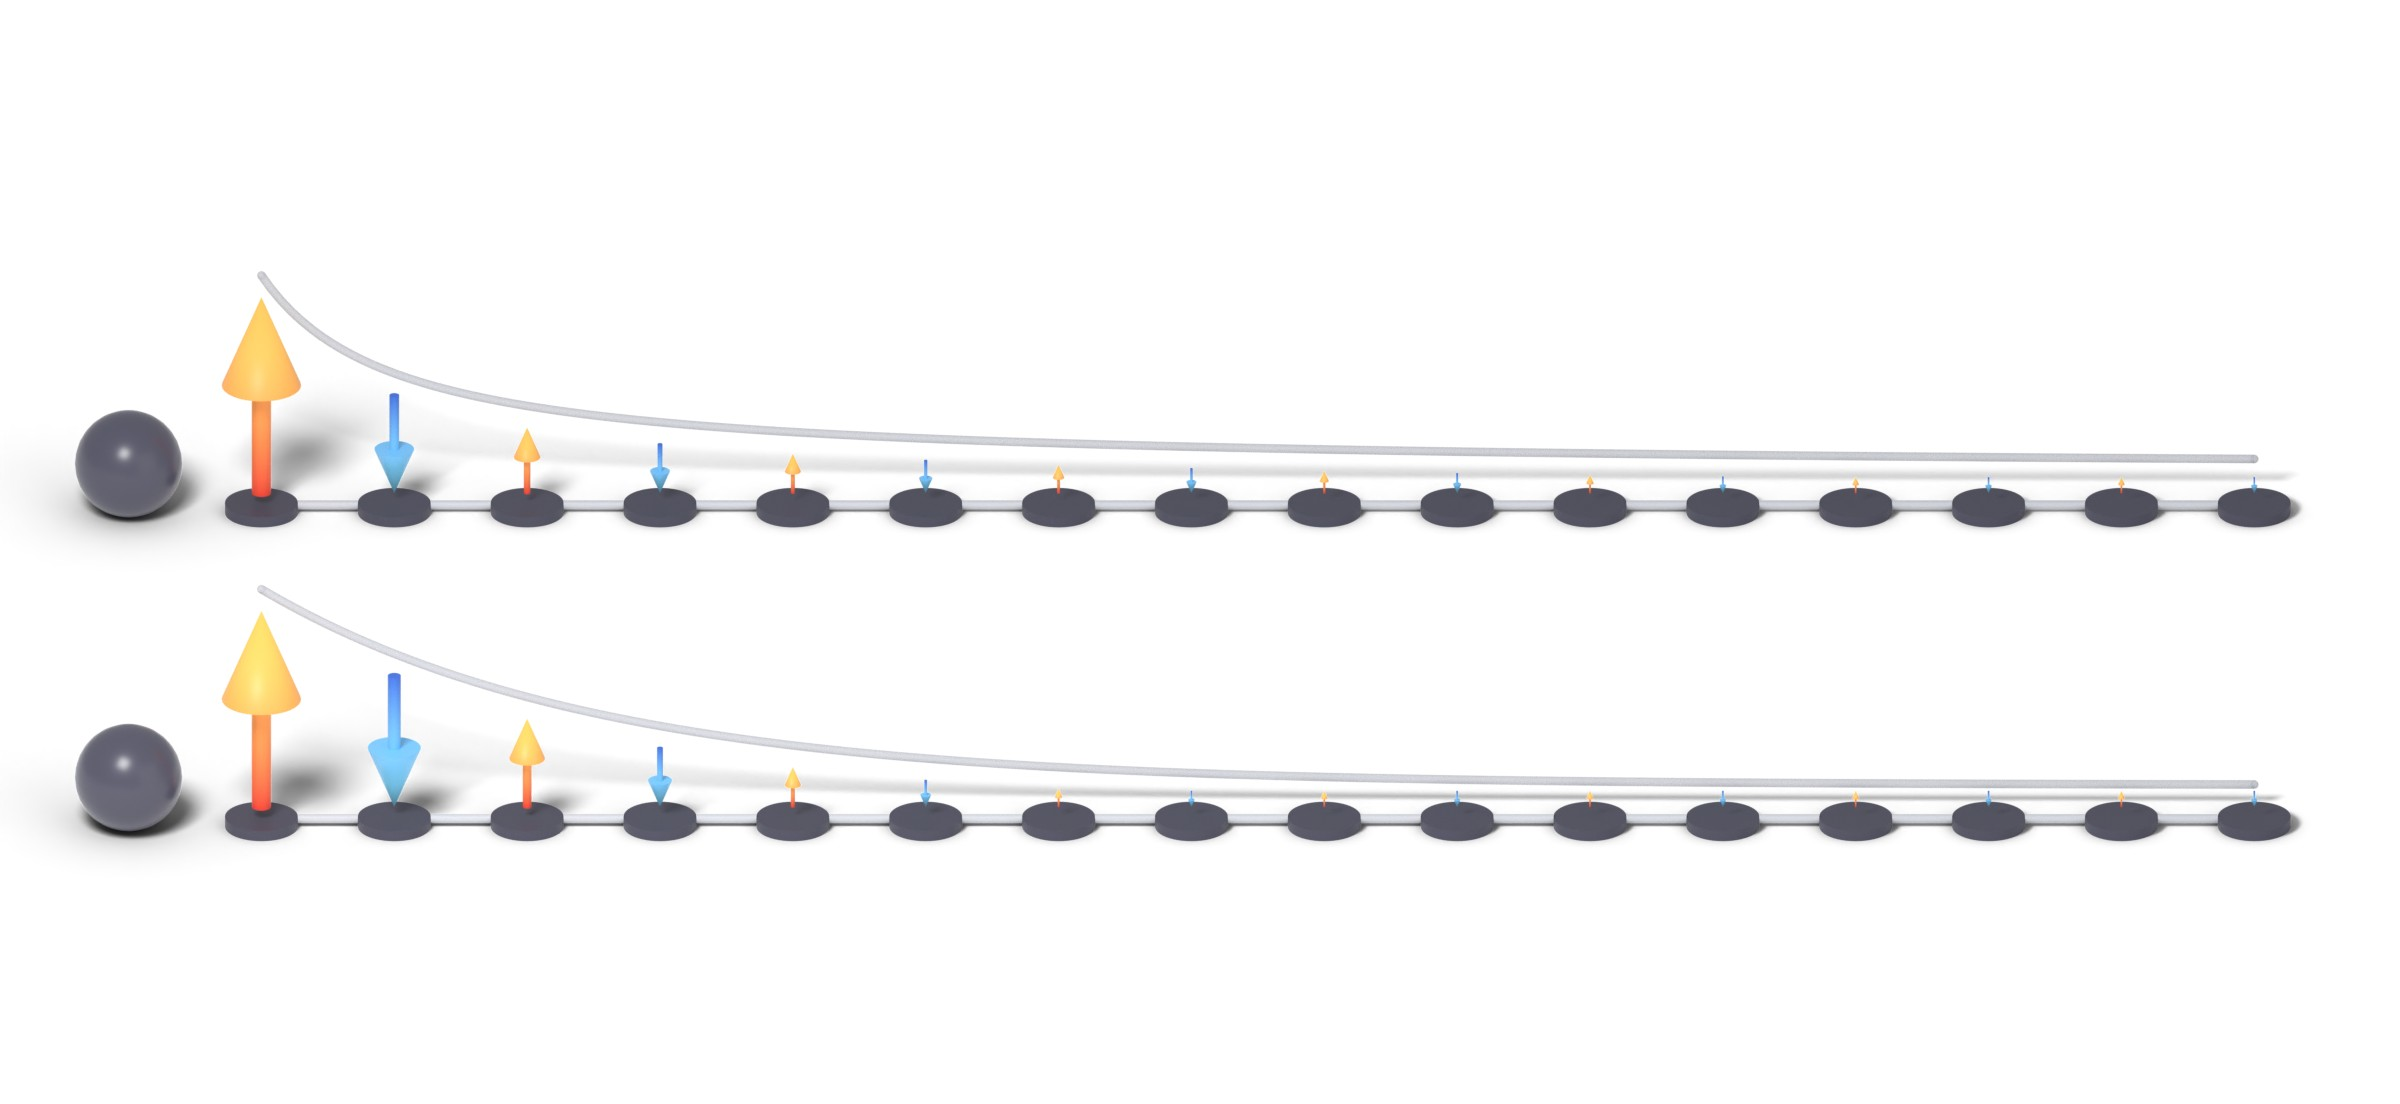
\includegraphics[width=\figw]{../blender/out/s09f05_decay_chains.jpg}};
    % written by build_figure.sh; the painted part of the image
\path (0.0083\figw,0.1013\figw) rectangle (0.9600\figw,0.3471\figw);

    %% written by figlib.py; x and y in units of the image width
\coordinate (chainsapanel) at (0.0134\figw,0.3688\figw);
\coordinate (chainsaenv) at (0.2750\figw,0.3167\figw);
\coordinate (chainsbpanel) at (0.0134\figw,0.2380\figw);
\coordinate (chainsbenv) at (0.2750\figw,0.1859\figw);

    \node[pnl, anchor=south east] at (chainsbpanel) {(a)};
    \node[pnl, anchor=south east] at ($(chainsapanel)!2!(chainsbpanel)$) {(b)};
    \node[lbl, anchor=south west, text=aqmmuted] at (chainsaenv) {$1/n$, $S=\tfrac12$};
    \node[lbl, anchor=south west, text=aqmmuted] at (chainsbenv) {$e^{-n/\xi}$, $S=1$};
  \end{scope}
  \begin{scope}[shift={(9.65cm,0.00cm)}]
    \setlength{\figw}{5.40cm}
    \node[overlay, anchor=south west, inner sep=0pt] at (0,0)
      {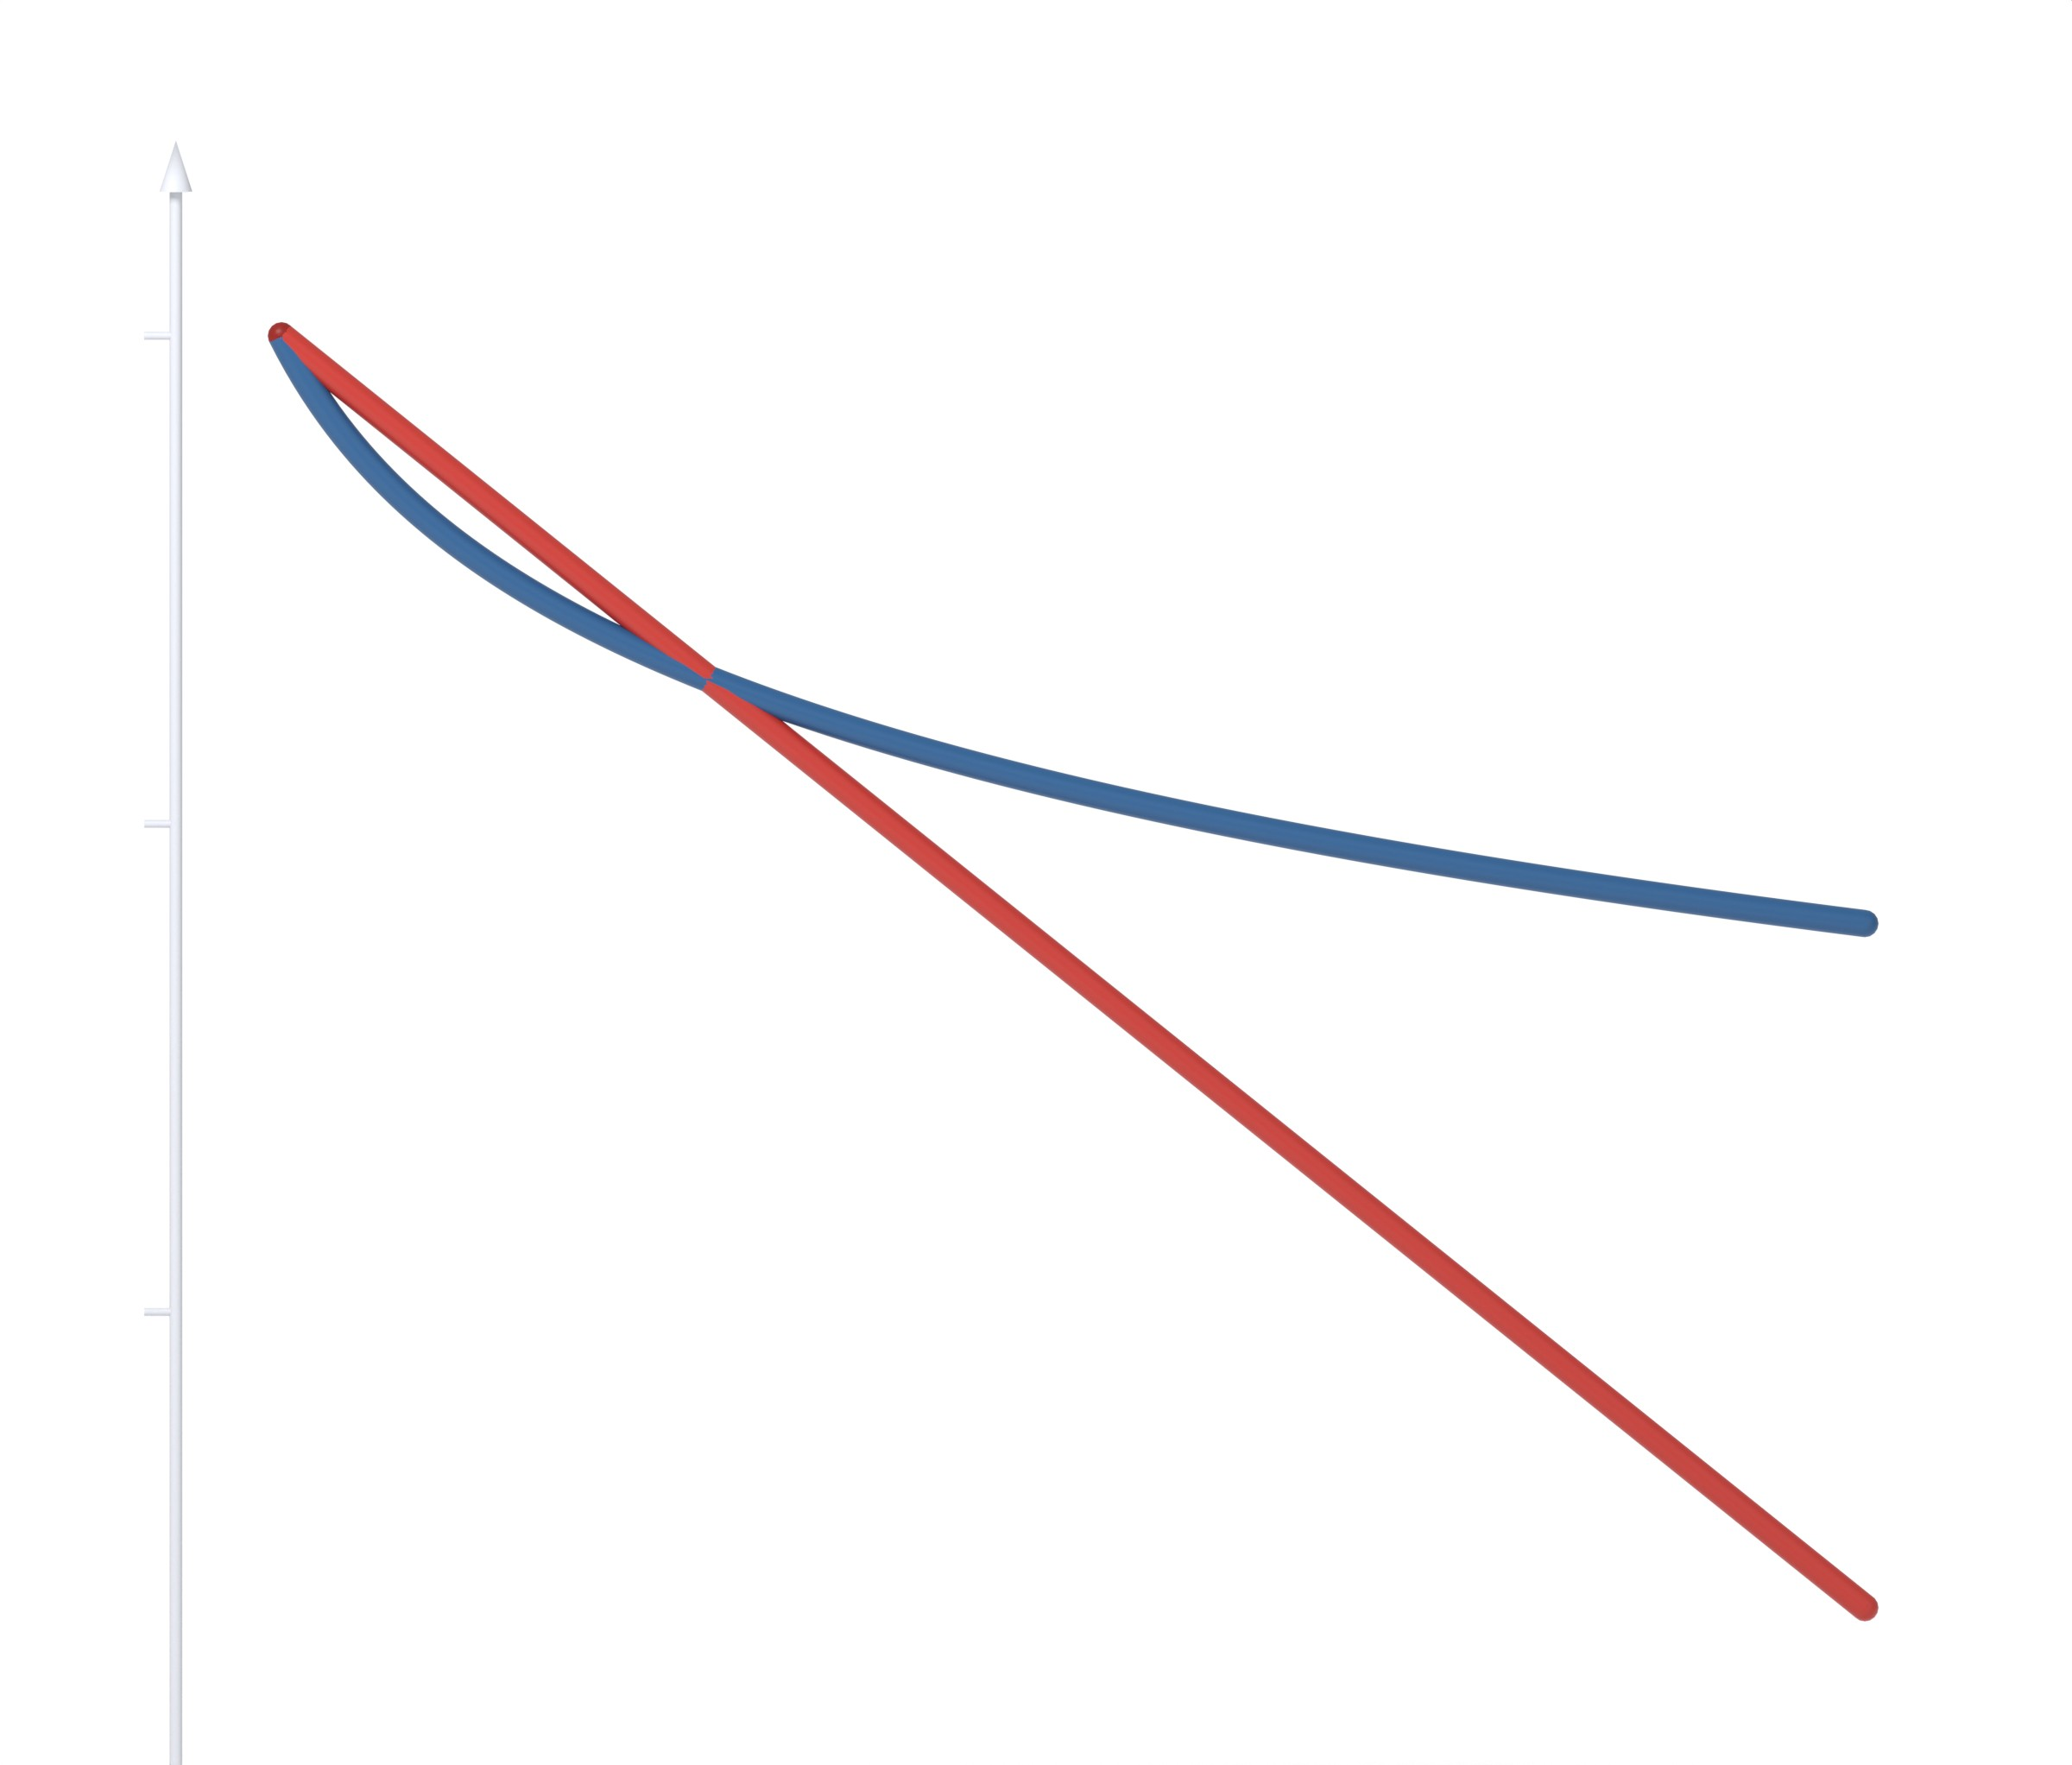
\includegraphics[width=\figw]{../blender/out/s09f05_decay_log.jpg}};
    % written by build_figure.sh; the painted part of the image
\path (0.0696\figw,0.0013\figw) rectangle (0.9067\figw,0.7837\figw);

    %% written by figlib.py; x and y in units of the image width
\coordinate (logd0) at (0.0696\figw,0.6896\figw);
\coordinate (logd1) at (0.0696\figw,0.4541\figw);
\coordinate (logd2) at (0.0696\figw,0.2186\figw);
\coordinate (logd3) at (0.0696\figw,-0.0170\figw);
\coordinate (logn) at (0.9764\figw,-0.0170\figw);
\coordinate (logy) at (0.0849\figw,0.7838\figw);
\coordinate (logpl) at (0.9000\figw,0.4060\figw);
\coordinate (logex) at (0.4670\figw,0.4237\figw);
\coordinate (logpanel) at (0.0340\figw,0.8192\figw);

    \node[pnl, anchor=south west] at (logpanel) {(c)};
    \node[lbl, anchor=east] at (logd0) {$1$};
    \foreach \d in {1,2,3} { \node[lbl, anchor=east] at (logd\d) {$10^{-\d}$}; }
    \node[lbl, anchor=north east] at (logn) {$n$};
    \node[lbl, anchor=west] at (logy) {envelope};
    \node[lbl, anchor=south east, text=aqmaccent] at (logpl) {$1/n$};
    \node[lbl, anchor=north east, text=aqmbroken] at (logex) {$e^{-n/\xi}$};
  \end{scope}
\end{tikzpicture}
\end{document}
